% Created 2019-05-09 Thu 17:20
% Intended LaTeX compiler: pdflatex
\documentclass[10pt, compress, aspectratio=169, xcolor={table,usenames,dvipsnames}]{beamer}

\usepackage{booktabs}
\mode<beamer>{\usetheme[numbering=fraction, progressbar=none, titleformat=smallcaps, sectionpage=none]{metropolis}}
\usepackage{sourcecodepro}
\usepackage{booktabs}
\usepackage{array}
\usepackage{listings}
\usepackage{graphicx}
\usepackage[english]{babel}
\usepackage[scale=2]{ccicons}
\usepackage{url}
\usepackage{relsize}
\usepackage{amsmath}
\usepackage{bm}
\usepackage{wasysym}
\usepackage{ragged2e}
\usepackage{textcomp}
\usepackage{pgfplots}
\usepgfplotslibrary{dateplot}
\definecolor{Base}{HTML}{191F26}
\definecolor{Accent}{HTML}{790700}
\setbeamercolor{alerted text}{fg=Accent}
\setbeamercolor{frametitle}{bg=Base}
\setbeamercolor{normal text}{bg=black!2,fg=Base}
\setsansfont[BoldFont={Source Sans Pro Semibold},Numbers={OldStyle}]{Source Sans Pro}
\lstdefinelanguage{Julia}%
{morekeywords={abstract,struct,break,case,catch,const,continue,do,else,elseif,%
end,export,false,for,function,immutable,mutable,using,import,importall,if,in,%
macro,module,quote,return,switch,true,try,catch,type,typealias,%
while,<:,+,-,::,/},%
sensitive=true,%
alsoother={$},%
morecomment=[l]\#,%
morecomment=[n]{\#=}{=\#},%
morestring=[s]{"}{"},%
morestring=[m]{'}{'},%
}[keywords,comments,strings]%
\lstset{ %
backgroundcolor={},
basicstyle=\ttfamily\scriptsize,
breakatwhitespace=true,
breaklines=true,
captionpos=n,
commentstyle=\color{Accent},
extendedchars=true,
frame=n,
keywordstyle=\color{Accent},
language=R,
rulecolor=\color{black},
showspaces=false,
showstringspaces=false,
showtabs=false,
stepnumber=2,
stringstyle=\color{gray},
tabsize=2,
}
\renewcommand*{\UrlFont}{\ttfamily\smaller\relax}
\graphicspath{{../../img/}}
\addtobeamertemplate{block begin}{}{\justifying}
\usetheme{default}
\author{\footnotesize \alert{Pedro Bruel}, Steven Quinito Masnada, Brice Videau, Arnaud Legrand, Jean-Marc Vincent, Alfredo Goldman}
\date{\scriptsize \today}
\title{Autotuning under Tight Budget Constraints:  \\ A Design of Experiments Approach}
\hypersetup{
 pdfauthor={\footnotesize \alert{Pedro Bruel}, Steven Quinito Masnada, Brice Videau, Arnaud Legrand, Jean-Marc Vincent, Alfredo Goldman},
 pdftitle={Autotuning under Tight Budget Constraints:  \\ A Design of Experiments Approach},
 pdfkeywords={},
 pdfsubject={},
 pdfcreator={Emacs 26.2 (Org mode 9.2.2)},
 pdflang={English}}
\begin{document}

\maketitle
\begin{frame}{Outline}
\tableofcontents
\end{frame}


\section{Autotuning}
\label{sec:org72775da}
\begin{frame}[label={sec:orgbd081e1},fragile]{Autotuning: Optimizing Program Configurations}
 \begin{columns}
\begin{column}{0.5\columnwidth}
\begin{block}{Architectures for High Performance Computing}
\begin{center}
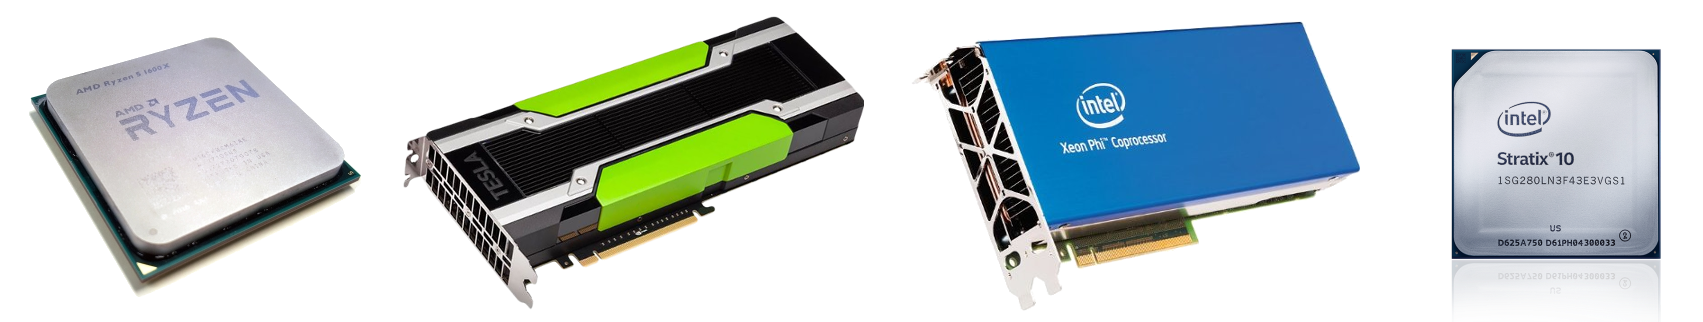
\includegraphics[width=.9\linewidth]{../../../img/architectures.png}
\end{center}

How to write \alert{efficient code} for each of these?

\begin{block}{Autotuning}
\vspace{.2cm}

The process of \alert{automatically finding} a \alert{configuration} of a program that
optimizes an \alert{objective}
\end{block}
\end{block}
\end{column}

\begin{column}{0.5\columnwidth}
\begin{block}{Configurations}
\begin{itemize}
\item Program Configuration
\begin{itemize}
\item Algorithm, block size, \(\dots\)
\end{itemize}
\item Source code transformation
\begin{itemize}
\item Loop unrolling, tiling, rotation \(\dots\)
\end{itemize}
\item Compiler configuration
\begin{itemize}
\item \texttt{-O2}, vectorization, \(\dots\)
\end{itemize}
\item \(\dots\)

\vspace{-.2cm}
\end{itemize}

\begin{block}{Objectives}
\begin{itemize}
\item Execution time
\item Memory \& power consumption
\item \(\dots\)
\end{itemize}
\end{block}
\end{block}
\end{column}
\end{columns}
\end{frame}

\begin{frame}[label={sec:orgc323e6b}]{Autotuning: Search Spaces}
\begin{columns}
\begin{column}{0.4\columnwidth}
\begin{block}{Search Spaces}
\vspace{.2cm}

Represent the \alert{effect} of all possible
\alert{configurations} on the \alert{objectives}

Can be difficult to explore, with multiple \alert{local optima}
and \alert{undefined regions}
\end{block}
\end{column}

\begin{column}{0.6\columnwidth}
\begin{center}
\begin{center}
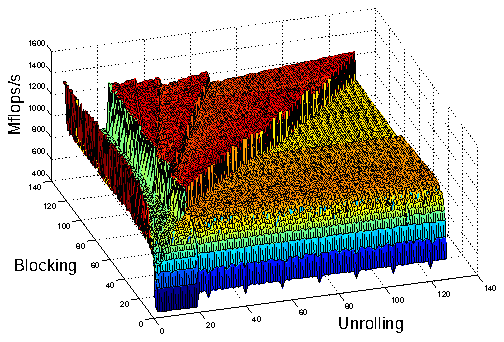
\includegraphics[width=.9\linewidth]{../../../img/seymour2008comparison.pdf}
\end{center}

\alert{Unrolling}, \alert{blocking} and \alert{Mflops/s} for \alert{matrix multiplication}

\vspace{.1cm}

\scriptsize{Seymour K, You H, Dongarra J. A comparison of search heuristics for empirical code optimization. InCLUSTER 2008 Oct 1 (pp. 421-429)}
\end{center}
\end{column}
\end{columns}
\end{frame}

\begin{frame}[label={sec:org311e0ec}]{Autotuning: Exploring Search Spaces}
\begin{columns}
\begin{column}{0.5\columnwidth}
\begin{block}{Issue 1: \alert{Exponential Growth}}
\vspace{.2cm}

\alert{Simple factors} can generate \alert{large spaces}:

\begin{itemize}
\item 30 \alert{boolean} factors \(\rightarrow\) \(2^{30}\) combinations
\end{itemize}

\begin{block}{Issue 2: \alert{Geometry}}
\begin{itemize}
\item \alert{Discrete} or \alert{continous} factors
\item \alert{``Smoothness''}
\item \alert{Interactions} between factors
\end{itemize}
\end{block}
\end{block}
\end{column}

\begin{column}{0.5\columnwidth}
\begin{block}{Issue 3: \alert{Measurement Time}}
\vspace{.2cm}

\begin{itemize}
\item \alert{Compile} time:
\begin{itemize}
\item Industrial \alert{FPGA} applications
\item Hardware and software \alert{co-design}
\end{itemize}
\item \alert{Execution} time:
\begin{itemize}
\item \alert{Benchmark} vs. \alert{real applications}
\end{itemize}
\end{itemize}
\end{block}
\end{column}
\end{columns}
\end{frame}
\begin{frame}[label={sec:org41a3a87}]{Autotuning: Multiple Approaches}
\begin{columns}
\begin{column}{0.5\columnwidth}
\begin{block}{Popular Approaches}
\footnotesize
\begin{itemize}
\item \colorbox{red!25}{Exhaustive}
\item \colorbox{green!25}{Meta-Heuristics}
\item \colorbox{cyan!25}{Machine Learning}
\end{itemize}
\normalsize

\vspace{-.4cm}

\begin{table}
    \centering
    \scriptsize
    \begin{tabular}{@{}lll@{}}
        \toprule
        System & Domain & Approach \\ \midrule
        \rowcolor{red!25} ATLAS & Dense Linear Algebra & Exhaustive\\ \addlinespace
        \rowcolor{green!25} INSIEME & Compiler & Genetic Algorithm \\
        \rowcolor{green!25} Active Harmony & Runtime & Nelder-Mead \\
        \rowcolor{green!25} ParamILS & Domain-Agnostic & Stochastic Local Search \\
        \rowcolor{green!25} OPAL & Domain-Agnostic & Direct Search \\
        \rowcolor{green!25} OpenTuner & Domain-Agnostic & Ensemble \\ \addlinespace
        \rowcolor{cyan!25} MILEPOST GCC & Compiler & Machine Learning \\
        \rowcolor{cyan!25} Apollo & GPU kernels & Decision Trees \\ \addlinespace
        \bottomrule
    \end{tabular}
\end{table}

\end{block}
\end{column}

\begin{column}{0.5\columnwidth}
\begin{block}{Main Issues}
\begin{itemize}
\item These approaches \alert{assume}:
\begin{itemize}
\item A \alert{large number of function evaluations}
\item Seach space \alert{``smoothness''}
\item Good solutions are \alert{reachable}
\end{itemize}
\item After optimizing:
\begin{itemize}
\item \alert{Learn ``nothing''} about the search space
\item \alert{Can't explain} why optimizations work
\end{itemize}
\end{itemize}
\begin{block}{Our Approach}
\begin{itemize}
\item \alert{Design of Experiments} (\alert{DoE})
\end{itemize}
\end{block}
\end{block}
\end{column}
\end{columns}
\end{frame}
\section{Design of Experiments}
\label{sec:org77bd7a3}
\begin{frame}[label={sec:org4ed68ef}]{Design of Experiments}
\begin{columns}
\begin{column}{0.5\columnwidth}
\begin{block}{Factors, Levels, Experiments \& Designs}
\vspace{.2cm}

\begin{itemize}
\item \alert{Factors}: program \alert{parameters}
\item \alert{Levels}: possible factor \alert{values}
\item \alert{Experiment}: setting each factor to a level
\item \alert{Design}: a \alert{selection} of experiments to \alert{run}
\item \alert{Performance Model}: guides \alert{selection}
\end{itemize}

\begin{block}{Analysis}
\vspace{.2cm}

\alert{Experiment results} can be used to:

\begin{itemize}
\item Identify \alert{relevant parameters}
\item Fit a \alert{regression model}
\end{itemize}
\end{block}
\end{block}
\end{column}

\begin{column}{0.5\columnwidth}
\vspace{.4cm}
\begin{center}

A \alert{small design} for \(7\) \alert{2-level factors}:

\end{center}

\begin{table}[]
    \centering
    \begin{tabular}{@{\kern\tabcolsep}cccccccc@{\kern\tabcolsep}}
        \toprule
        Run & A & B & C & D & E & F & G \\ \midrule
        \cellcolor{gray!18}1 & \cellcolor{green!25}1 & \cellcolor{red!25}-1 & \cellcolor{green!25}1 & \cellcolor{red!25}-1 & \cellcolor{red!25}-1 & \cellcolor{green!25}1 & \cellcolor{green!25}1 \\
        \cellcolor{gray!18}2 & \cellcolor{green!25}1 & \cellcolor{green!25}1 & \cellcolor{green!25}1 & \cellcolor{red!25}-1 & \cellcolor{green!25}1 & \cellcolor{red!25}-1 & \cellcolor{red!25}-1 \\
        \cellcolor{gray!18}3 & \cellcolor{red!25}-1 & \cellcolor{green!25}1 & \cellcolor{red!25}-1 & \cellcolor{red!25}-1 & \cellcolor{green!25}1 & \cellcolor{green!25}1 & \cellcolor{green!25}1 \\
        \cellcolor{gray!18}4 & \cellcolor{red!25}-1 & \cellcolor{green!25}1 & \cellcolor{green!25}1 & \cellcolor{green!25}1 & \cellcolor{red!25}-1 & \cellcolor{green!25}1 & \cellcolor{red!25}-1 \\
        \cellcolor{gray!18}5 & \cellcolor{green!25}1 & \cellcolor{red!25}-1 & \cellcolor{red!25}-1 & \cellcolor{green!25}1 & \cellcolor{green!25}1 & \cellcolor{green!25}1 & \cellcolor{red!25}-1 \\
        \cellcolor{gray!18}6 & \cellcolor{green!25}1 & \cellcolor{green!25}1 & \cellcolor{red!25}-1 & \cellcolor{green!25}1 & \cellcolor{red!25}-1 & \cellcolor{red!25}-1 & \cellcolor{green!25}1 \\
        \cellcolor{gray!18}7 & \cellcolor{red!25}-1 & \cellcolor{red!25}-1 & \cellcolor{green!25}1 & \cellcolor{green!25}1 & \cellcolor{green!25}1 & \cellcolor{red!25}-1 & \cellcolor{green!25}1 \\
        \cellcolor{gray!18}8 & \cellcolor{red!25}-1 & \cellcolor{red!25}-1 & \cellcolor{red!25}-1 & \cellcolor{red!25}-1 & \cellcolor{red!25}-1 & \cellcolor{red!25}-1 & \cellcolor{red!25}-1  \\ \bottomrule
    \end{tabular}
\end{table}

\end{column}
\end{columns}
\end{frame}

\begin{frame}[label={sec:orga447f58}]{Applying Design of Experiments to Autotuning}
\begin{columns}
\begin{column}{0.5\columnwidth}
\begin{block}{Our Approach}
\vspace{.2cm}

We are using:

\begin{itemize}
\item \alert{Efficient experimental designs} to overcome issues related to \alert{exponential growth}, \alert{geometry}, and \alert{measurement time}
\item \alert{Analysis of variance} to find \alert{relevant parameters}
\item \alert{User input} to guide optimization
\end{itemize}

\begin{block}{Validation}
\begin{itemize}
\item \alert{Source code transformations}
\item \alert{GPU Laplacian} kernel
\item HPC kernels from the \alert{SPAPT benchmark}
\end{itemize}
\end{block}
\end{block}
\end{column}

\begin{column}{0.5\columnwidth}
\begin{block}{Design Requirements}
\begin{itemize}
\item Support a large number of factors (\alert{Exponential Growth})
\item Support numerical and categorical factors (\alert{Geometry})
\item Minimize function evaluations (\alert{Measurement Time})
\end{itemize}

\begin{block}{D-Optimal Designs}
\begin{itemize}
\item Minimize \alert{variance} of \alert{regression coefficient estimators}
\item Supports different factor \alert{types} and \alert{numbers}
\end{itemize}
\end{block}
\end{block}
\end{column}
\end{columns}
\end{frame}

\begin{frame}[label={sec:orgd15074e},fragile]{D-Optimal Designs: Example}
 \begin{columns}
\begin{column}{0.6\columnwidth}
\begin{block}{Example}
% \(\mathbf{X} = \{x_1 = \{1, \dots, 5\}, x_2 = \{"A", "B", "C"\}\}\)
\begin{itemize}
\item Factors \& Levels:
\begin{align*}
\mathbf{X} = (x_1 = & \; (1, \dots, 5), \\
x_2 = & \; (``A", ``B", ``C"))
\end{align*}
\item Model: \(\mathbf{Y} = \mathbf{X}\bm{\beta} + \bm{\varepsilon}\)
\end{itemize}

\begin{block}{Source code}
\vspace{-.2cm}

\lstset{language=r,label= ,caption= ,captionpos=b,numbers=none}
\begin{lstlisting}
library(AlgDesign)

full_factorial <- gen.factorial(c(5, 3),
                      factors = c(2))

output <- optFederov(~ .,
                     full_factorial,
                     nTrials = 5)
\end{lstlisting}
\end{block}
\end{block}
\end{column}

\begin{column}{0.4\columnwidth}
\begin{block}{Output}
\vspace{-.2cm}
\scriptsize

\begin{verbatim}

$D
[1] 0.5656854

$A
[1] 3.90625

$Ge
[1] 0.512

$Dea
[1] 0.386

$design
   1    5    7    11   15
X1 "-2" " 2" "-1" "-2" " 2"
X2 "1"  "1"  "2"  "3"  "3"

$rows
[1]  1  5  7 11 15
\end{verbatim}


\normalsize
\end{block}
\end{column}
\end{columns}
\end{frame}
\begin{frame}[label={sec:org2075262}]{Design Efficiency}
\begin{columns}
\begin{column}{0.5\columnwidth}
\begin{block}{Linear Regression Model}
\vspace{.2cm}

The \alert{linear regression model}:
\begin{center}
\(y = \beta_{0} + \beta_{1}x_{1} + \dots + \beta_{k}x_{k} + \epsilon\)
\end{center}
We want to \alert{estimate} \(\beta_{0,\dots,k}\):

\begin{itemize}
\item Using \(n > k\) \alert{observations} \(y_{1,\dots,n}\)
\item \alert{Distinct} \(x_{i1,\dots,ik}, \; i = 1,\dots,n\)
\end{itemize}

\alert{Experiments} represented by:
\begin{center}
\(y_{i} = \beta_{0} + \beta_{1}x_{i1} + \dots + \beta_{k}x_{ik} + \epsilon_{i}\)
\end{center}
\end{block}
\end{column}
\begin{column}{0.5\columnwidth}
\begin{block}{Ordinary Least Squares Estimator \(\bm{\hat{\beta}}\)}
\begin{center}
\begin{equation*}
\bm{\hat{\beta}} = \left(\bm{X}^{\intercal}\bm{X}\right)^{-1}\bm{X}^{\intercal}\bm{Y}
\end{equation*}
\end{center}

The \alert{variance} of \(\bm{\hat{\beta}}\) is proportional to
the \alert{covariance matrix} \(\left(\bm{X}^{\intercal}\bm{X}\right)^{-1}\)

\begin{block}{Design Criteria using \(\left(\bm{X}^{\intercal}\bm{X}\right)^{-1}\)}
\begin{itemize}
\item \alert{D}: \alert{determinant}, minimizes generalized variance of \(\bm{\hat{\beta}}\)
\item \alert{A}: \alert{trace}, average variance of \(\bm{\hat{\beta}}\)
\end{itemize}
\end{block}
\end{block}
\end{column}
\end{columns}
\end{frame}
\begin{frame}[label={sec:org5122e5b}]{Comparing Sampling Strategies}
\begin{center}
\begin{center}
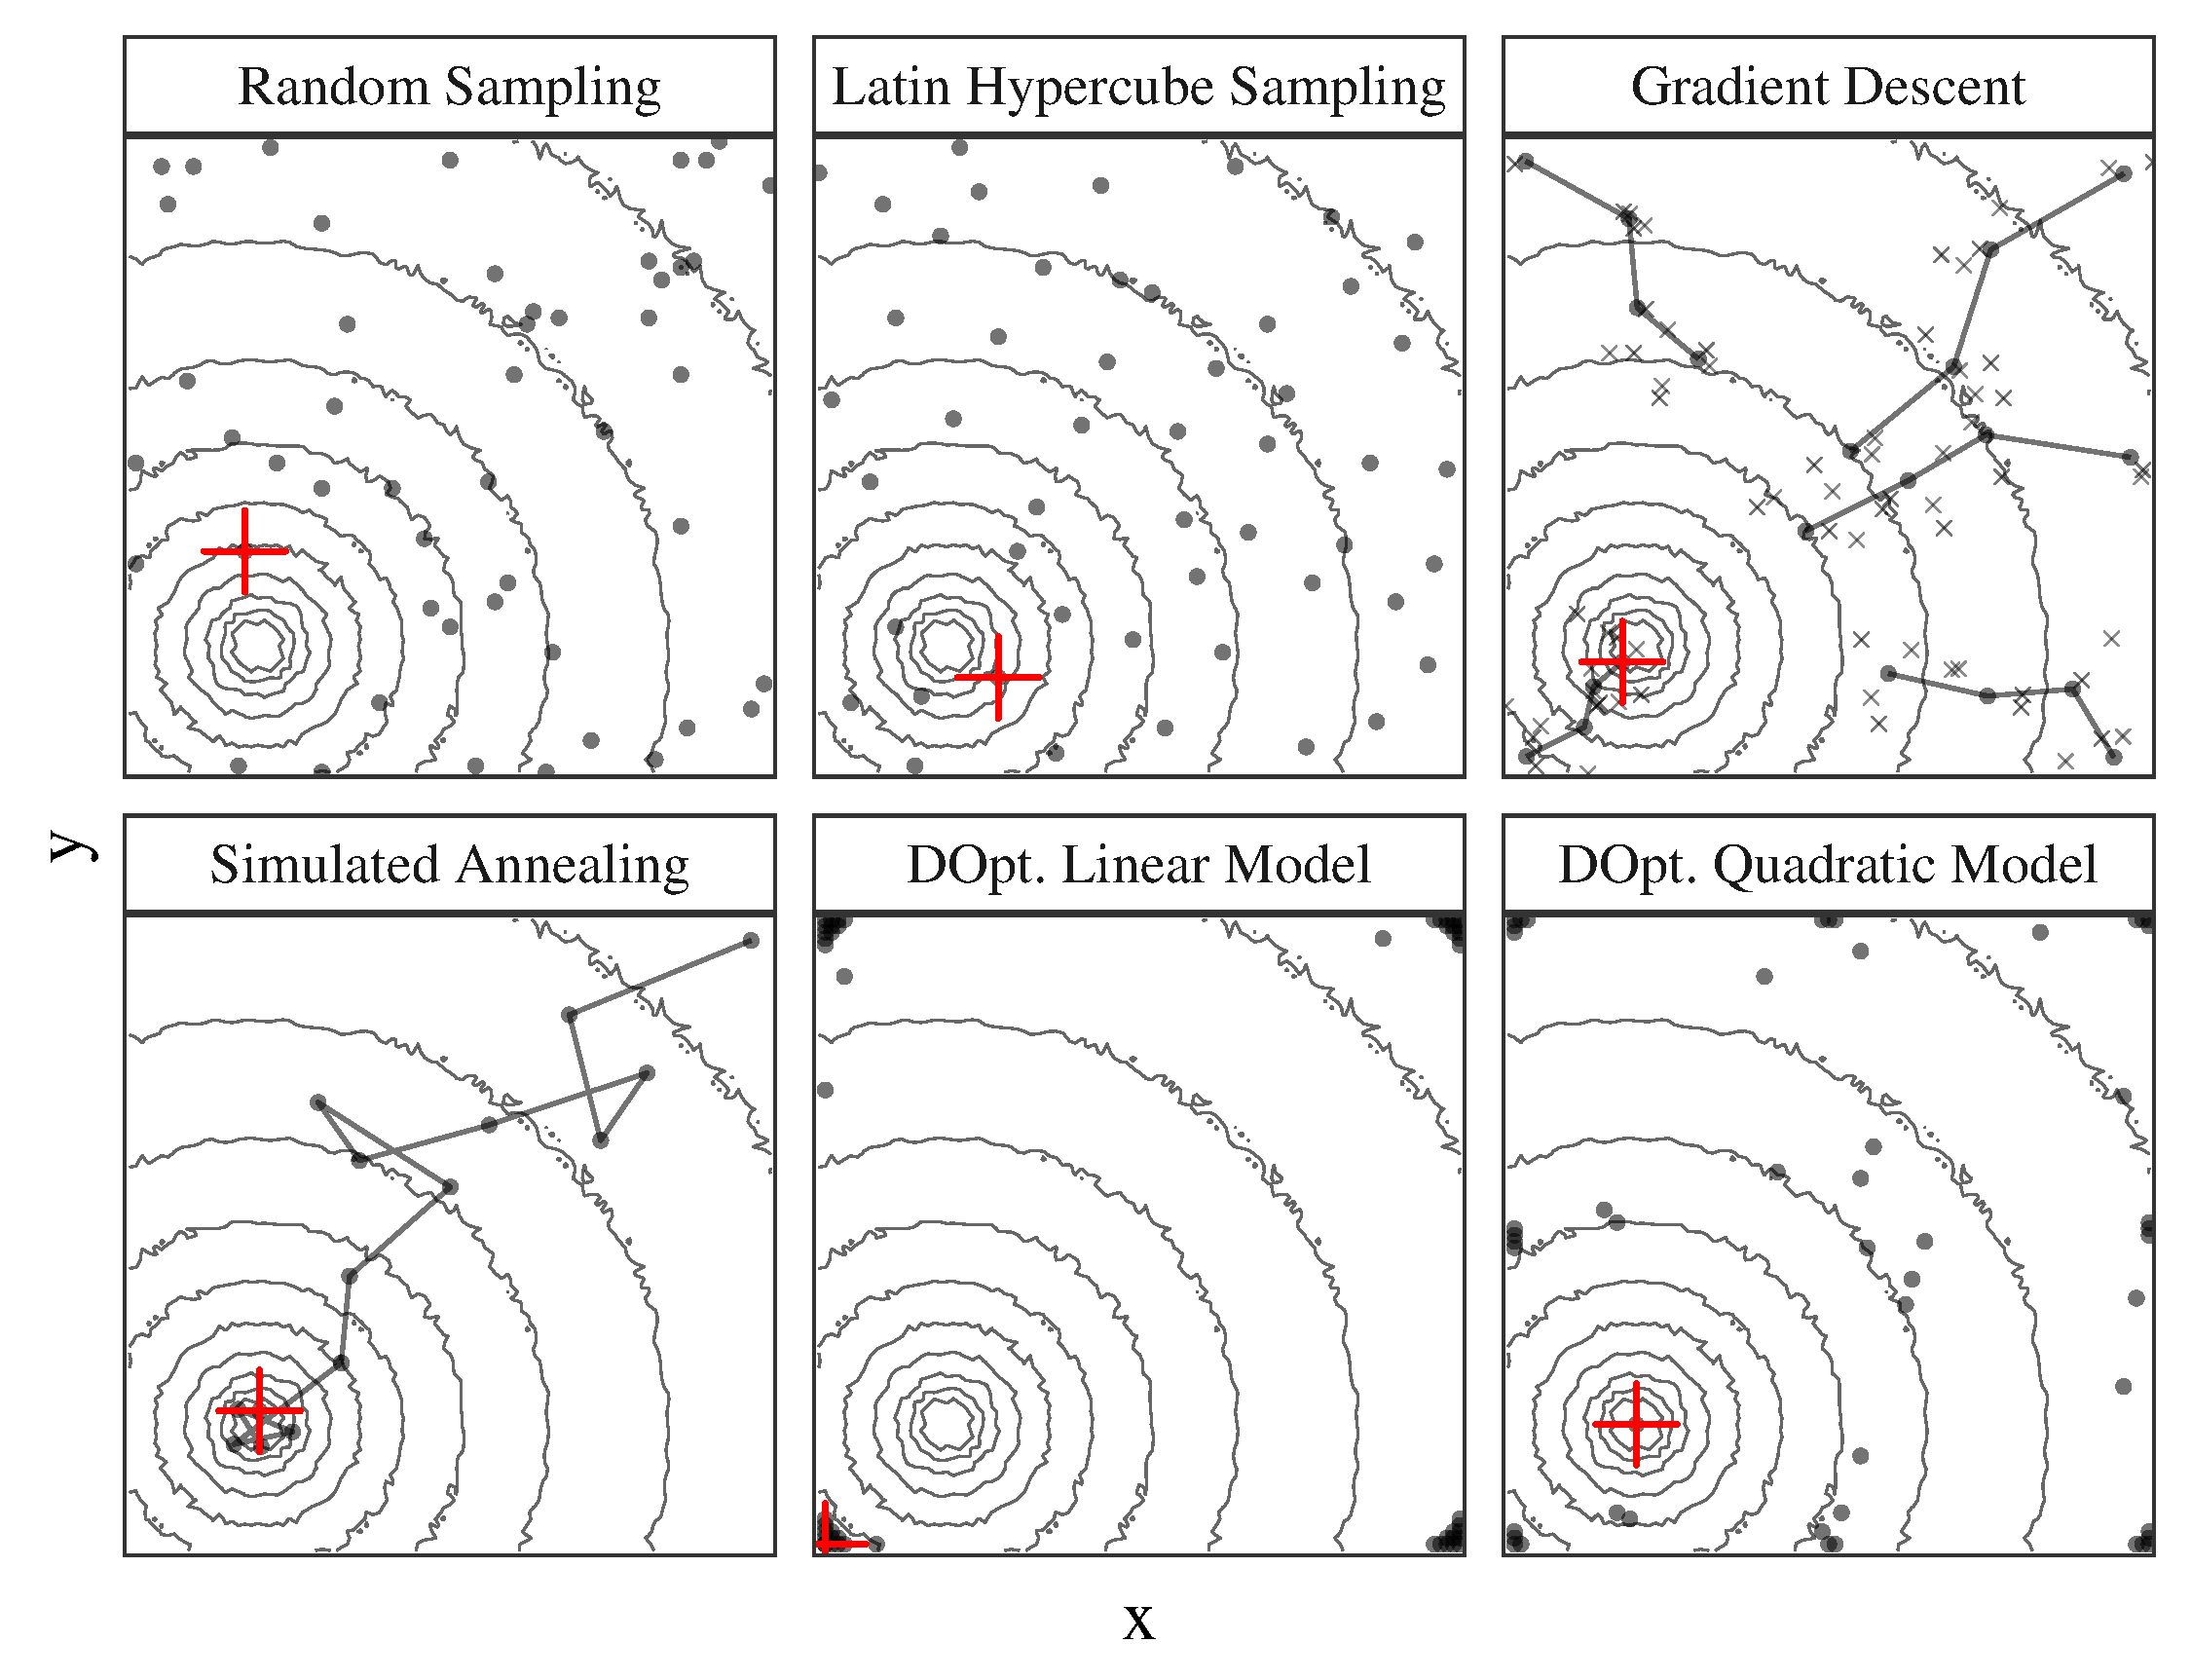
\includegraphics[width=.72\textwidth]{../../../img/sampling_comparison.pdf}
\end{center}
\end{center}
\end{frame}
\section{Our Approach}
\label{sec:orgccf7891}
\begin{frame}[label={sec:orgb534b8e}]{A Design of Experiments Approach to Autotuning}
\begin{center}
\begin{center}
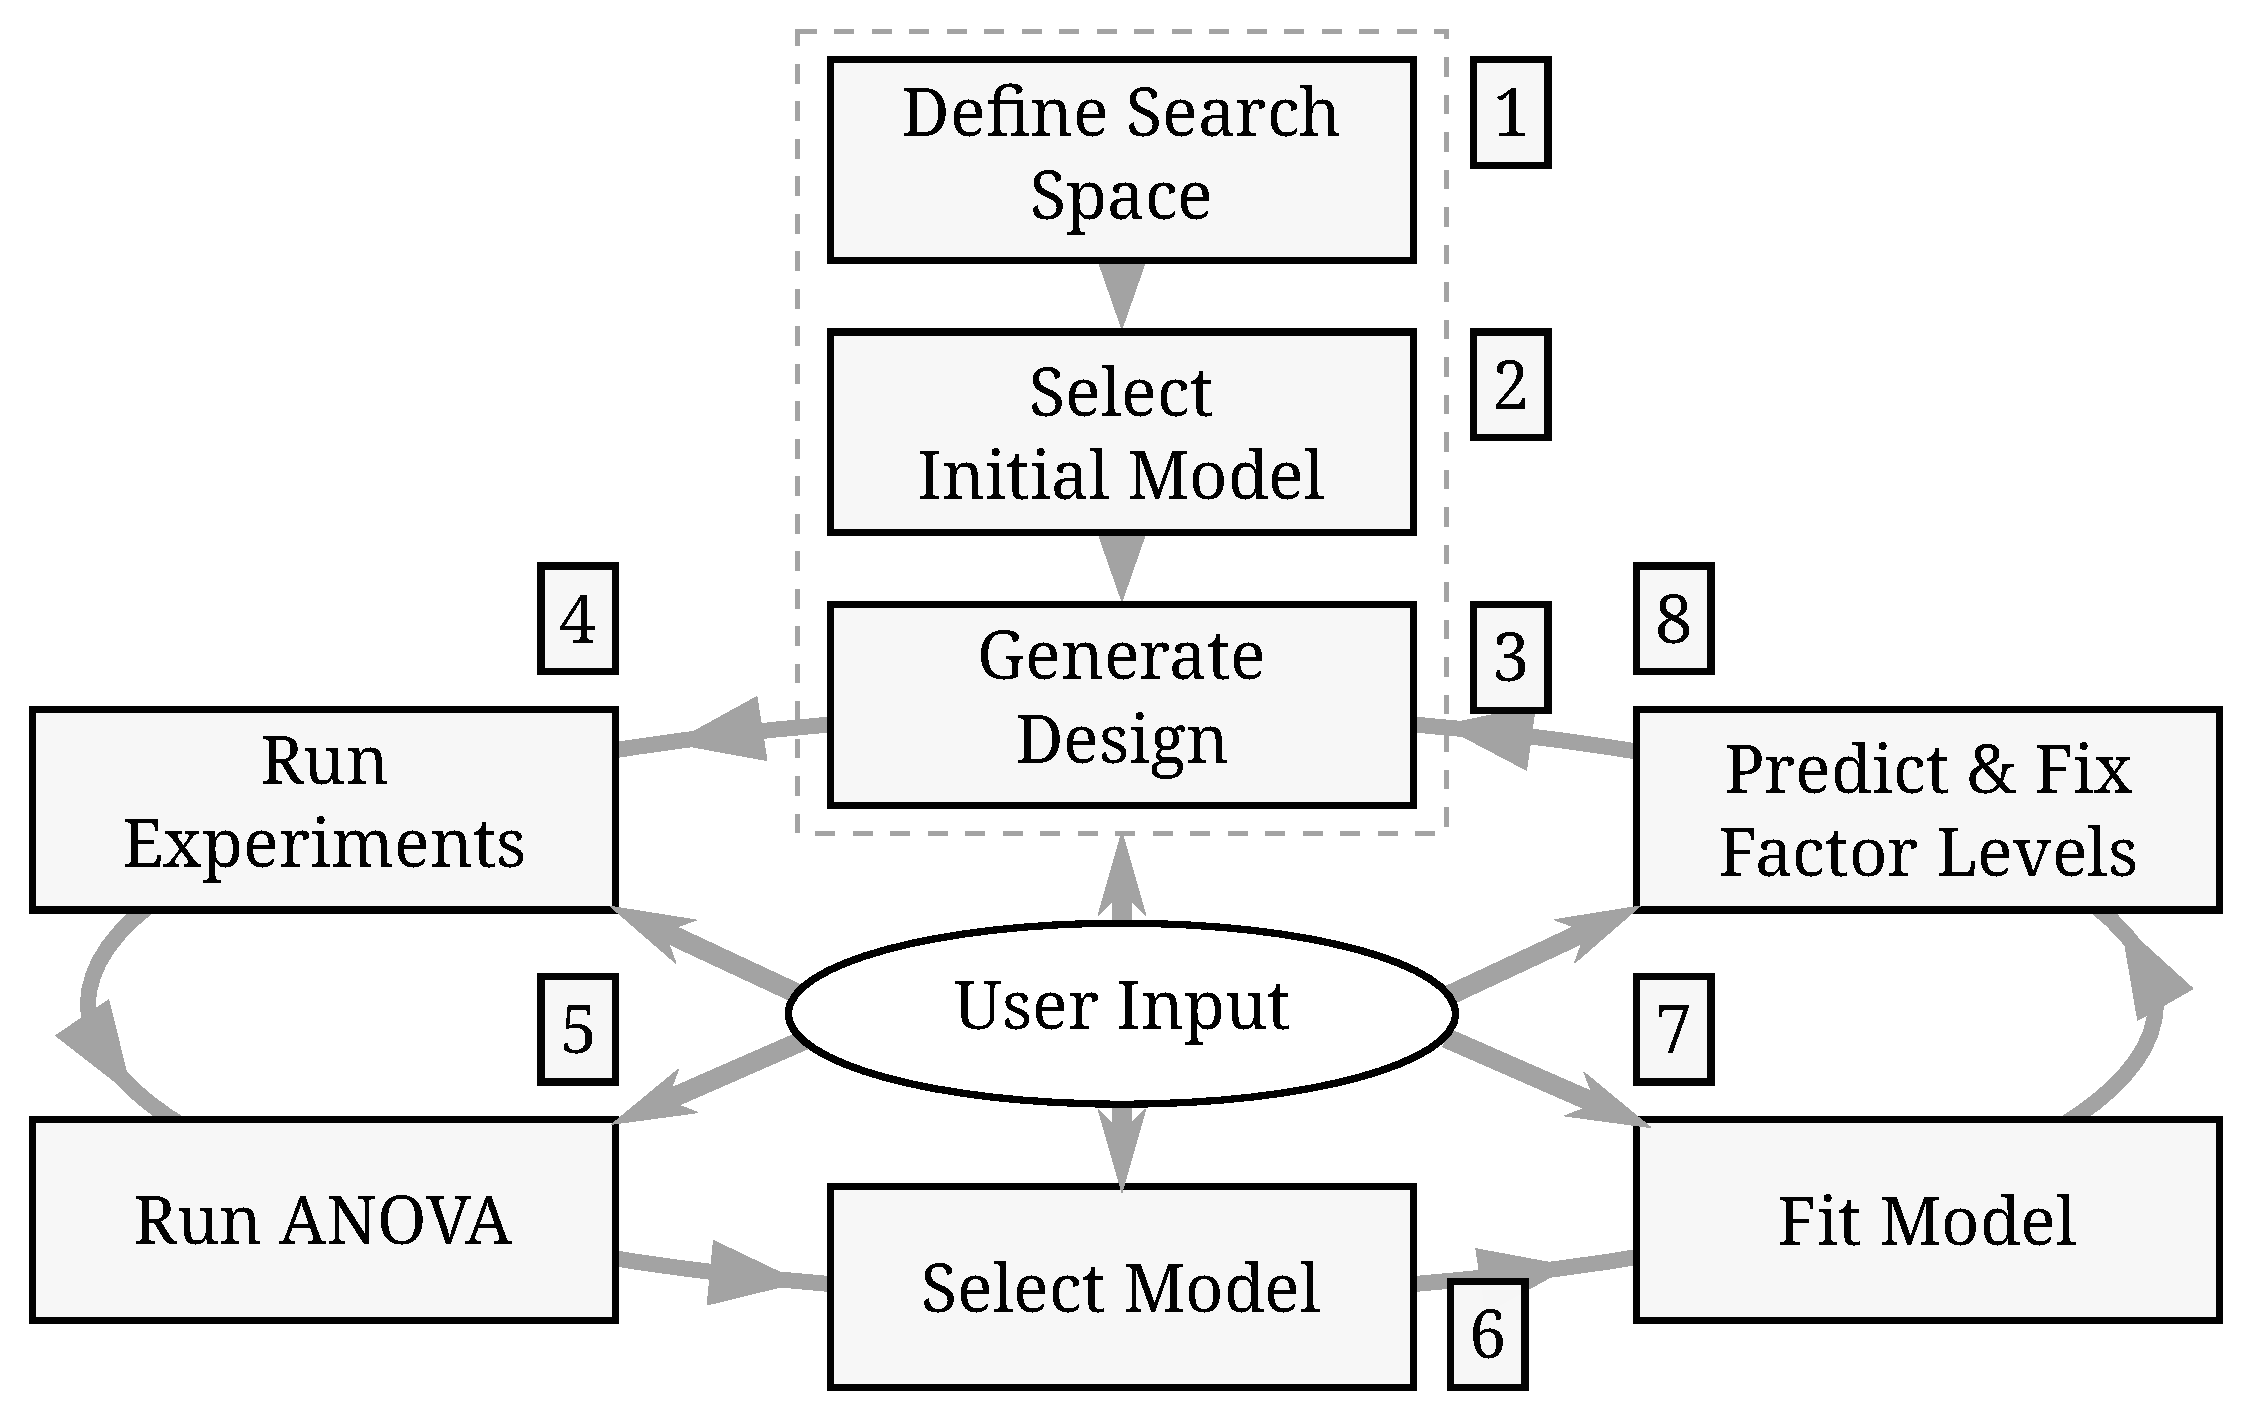
\includegraphics[width=.74\linewidth]{../../../img/doe_anova_strategy.pdf}
\end{center}

\vspace{-.2cm}
\end{center}
\end{frame}
\section{Results on a GPU Laplacian Kernel}
\label{sec:org720215b}
\begin{frame}[label={sec:orge980c02}]{GPU Laplacian Kernel: A Motivating Example}
\begin{columns}
\begin{column}{0.5\columnwidth}
\begin{block}{The Search Problem}
\begin{itemize}
\item Relatively \alert{small valid search space}
\item \alert{Completely evaluated}
\item Known \alert{global optimum}
\item Known \alert{model approximation}
\item \alert{Budget} of \alert{125 points}
\end{itemize}
\end{block}
\end{column}

\begin{column}{0.5\columnwidth}
\begin{block}{Initial Model}
\footnotesize
\begin{align*}
cost = & \; y\_component\_number + 1 / y\_component\_number \; + \\
& \; vector\_length + lws\_y + 1 / lws\_y \; + \\
& \; load\_overlap + temporary\_size \; + \\
& \; elements\_number + 1 / elements\_number \; + \\
& \; threads\_number + 1 / threads\_number
\end{align*}
\normalsize
\end{block}
\end{column}
\end{columns}

\begin{block}{Results}
\vspace{-.3cm}

\begin{center}
\begin{center}
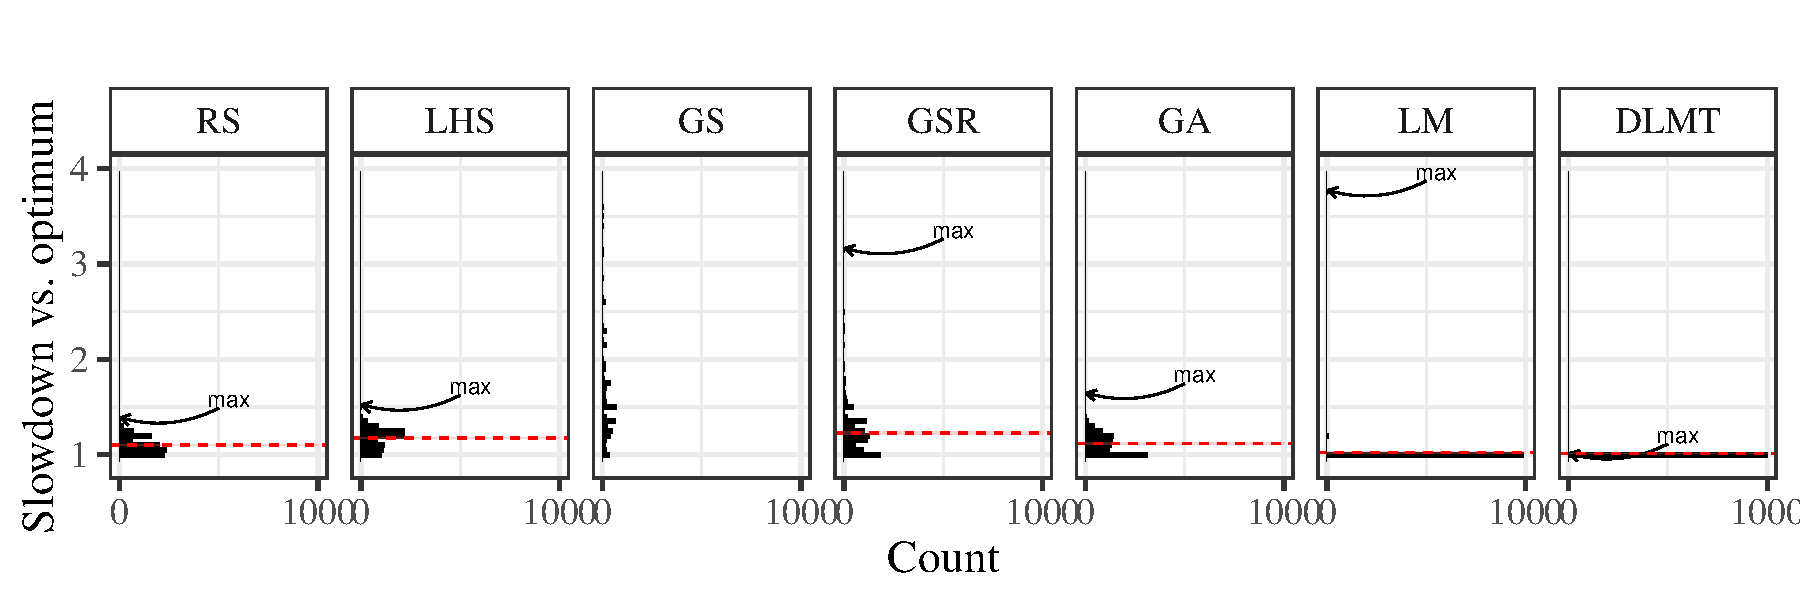
\includegraphics[width=.88\columnwidth]{../../../img/comparison_histogram.pdf}
\end{center}
\end{center}
\end{block}
\end{frame}

\begin{frame}[label={sec:orgcdafc7f}]{GPU Laplacian Kernel: A Motivating Example}
\begin{columns}
\begin{column}{0.5\columnwidth}
\begin{table}[ht]
\centering
\begingroup\small
\begin{tabular}{lrr}
  \hline
  & Mean & Max \\
  \hline
  RS & 120.00 & 125.00 \\
  LHS & 98.92 & 125.00 \\
  GS & 22.17 & 106.00 \\
  GSR & 120.00 & 120.00 \\
  GA & 120.00 & 120.00 \\
  LM & 119.00 & 119.00 \\
  DLMT & 54.84 & 56.00 \\
    \hline
\end{tabular}
\endgroup
\caption{Points used by applications}
\end{table}
\end{column}

\begin{column}{0.5\columnwidth}
\begin{block}{Summary}
\vspace{.2cm}

Our approach:

\begin{itemize}
\item Was \alert{always close to the optimum}
\item Used \alert{half of the budget}
\end{itemize}
\end{block}
\end{column}
\end{columns}
\end{frame}

\section{Results on the SPAPT Benchmark}
\label{sec:org89ec686}
\begin{frame}[label={sec:orgdb35555},fragile]{SPAPT: Search Problems in Automatic Performance Tuning}
 \begin{center}
\begin{table}[t]
\label{tab:org19b128e}
\centering
\scriptsize
\begin{tabular}{llll}
\toprule
Kernel & Operation & Factors & Size\\
\midrule
\texttt{atax} & Matrix transp. \& vector mult. & 18 & \(2.6 \times 10^{16}\)\\
\texttt{dgemv3} & Scalar, vector \& matrix mult. & 49 & \(3.8 \times 10^{36}\)\\
\texttt{gemver} & Vector mult. \& matrix add. & 24 & \(2.6 \times 10^{22}\)\\
\texttt{gesummv} & Scalar, vector, \& matrix mult. & 11 & \(5.3 \times 10^{9}\)\\
\texttt{hessian} & Hessian computation & 9 & \(3.7 \times 10^{7}\)\\
\texttt{mm} & Matrix multiplication & 13 & \(1.2 \times 10^{12}\)\\
\texttt{mvt} & Matrix vector product \& transp. & 12 & \(1.1 \times 10^{9}\)\\
\texttt{tensor} & Tensor matrix mult. & 20 & \(1.2 \times 10^{19}\)\\
\texttt{trmm} & Triangular matrix operations & 25 & \(3.7 \times 10^{23}\)\\
\texttt{bicg} & Subkernel of BiCGStab & 13 & \(3.2 \times 10^{11}\)\\
\texttt{lu} & LU decomposition & 14 & \(9.6 \times 10^{12}\)\\
\texttt{adi} & Matrix sub., mult., \& div. & 20 & \(6.0 \times 10^{15}\)\\
\texttt{jacobi} & 1-D Jacobi computation & 11 & \(5.3 \times 10^{9}\)\\
\texttt{seidel} & Matrix factorization & 15 & \(1.3 \times 10^{14}\)\\
\texttt{stencil3d} & 3-D stencil computation & 29 & \(9.7 \times 10^{27}\)\\
\texttt{correlation} & Correlation computation & 21 & \(4.5 \times 10^{17}\)\\
\bottomrule
\end{tabular}
\end{table}

\scriptsize{Balaprakash P, Wild SM, Norris B. SPAPT: Search problems in automatic performance tuning. Procedia Comp. Sci. 2012 Jan 1;9:1959-68.}
\end{center}
\end{frame}

\begin{frame}[label={sec:orgcb360d0}]{SPAPT: Preliminary Results}
\begin{center}
\begin{center}
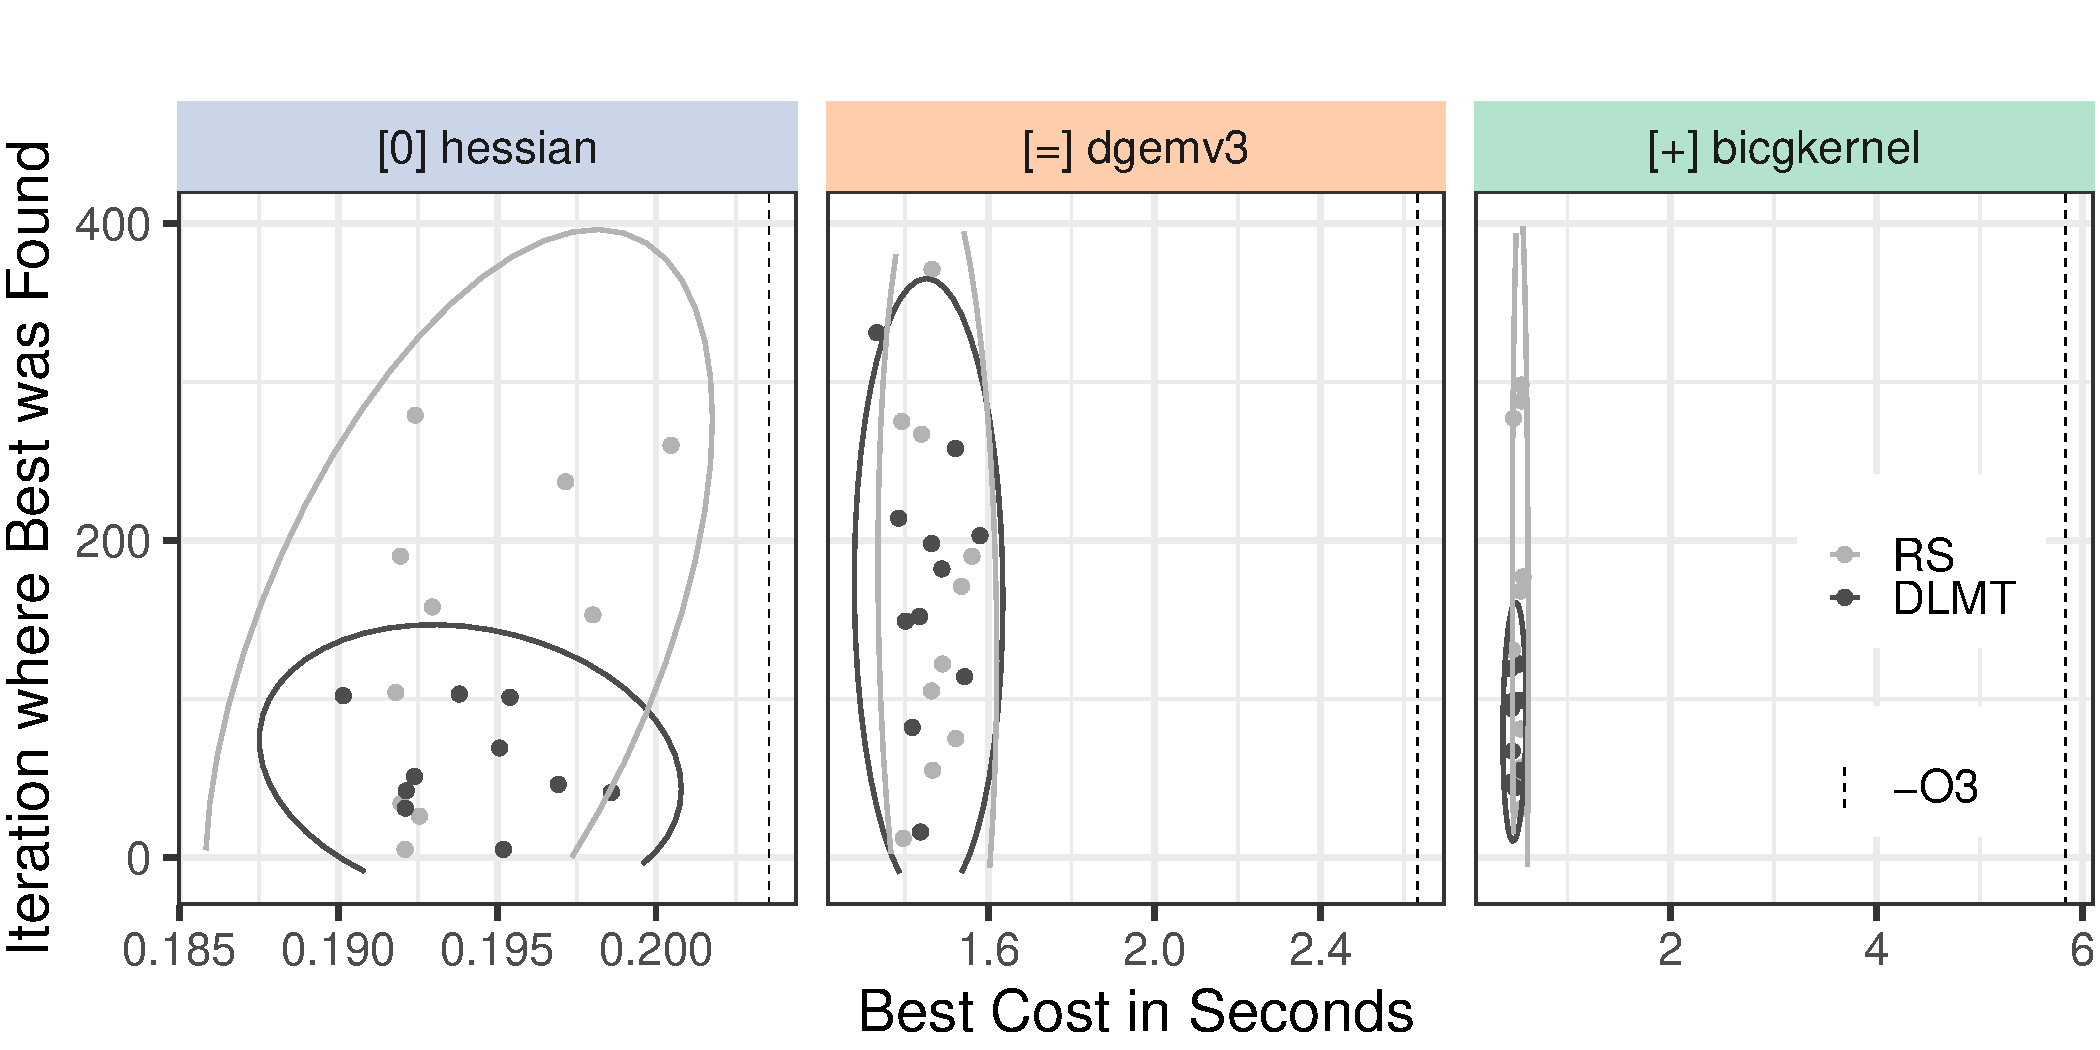
\includegraphics[width=.86\linewidth]{../../../img/iteration_best_comparison.pdf}
\end{center}
\end{center}
\end{frame}
\begin{frame}[label={sec:orgb791b8f}]{SPAPT: Preliminary Results}
\begin{center}
\begin{center}
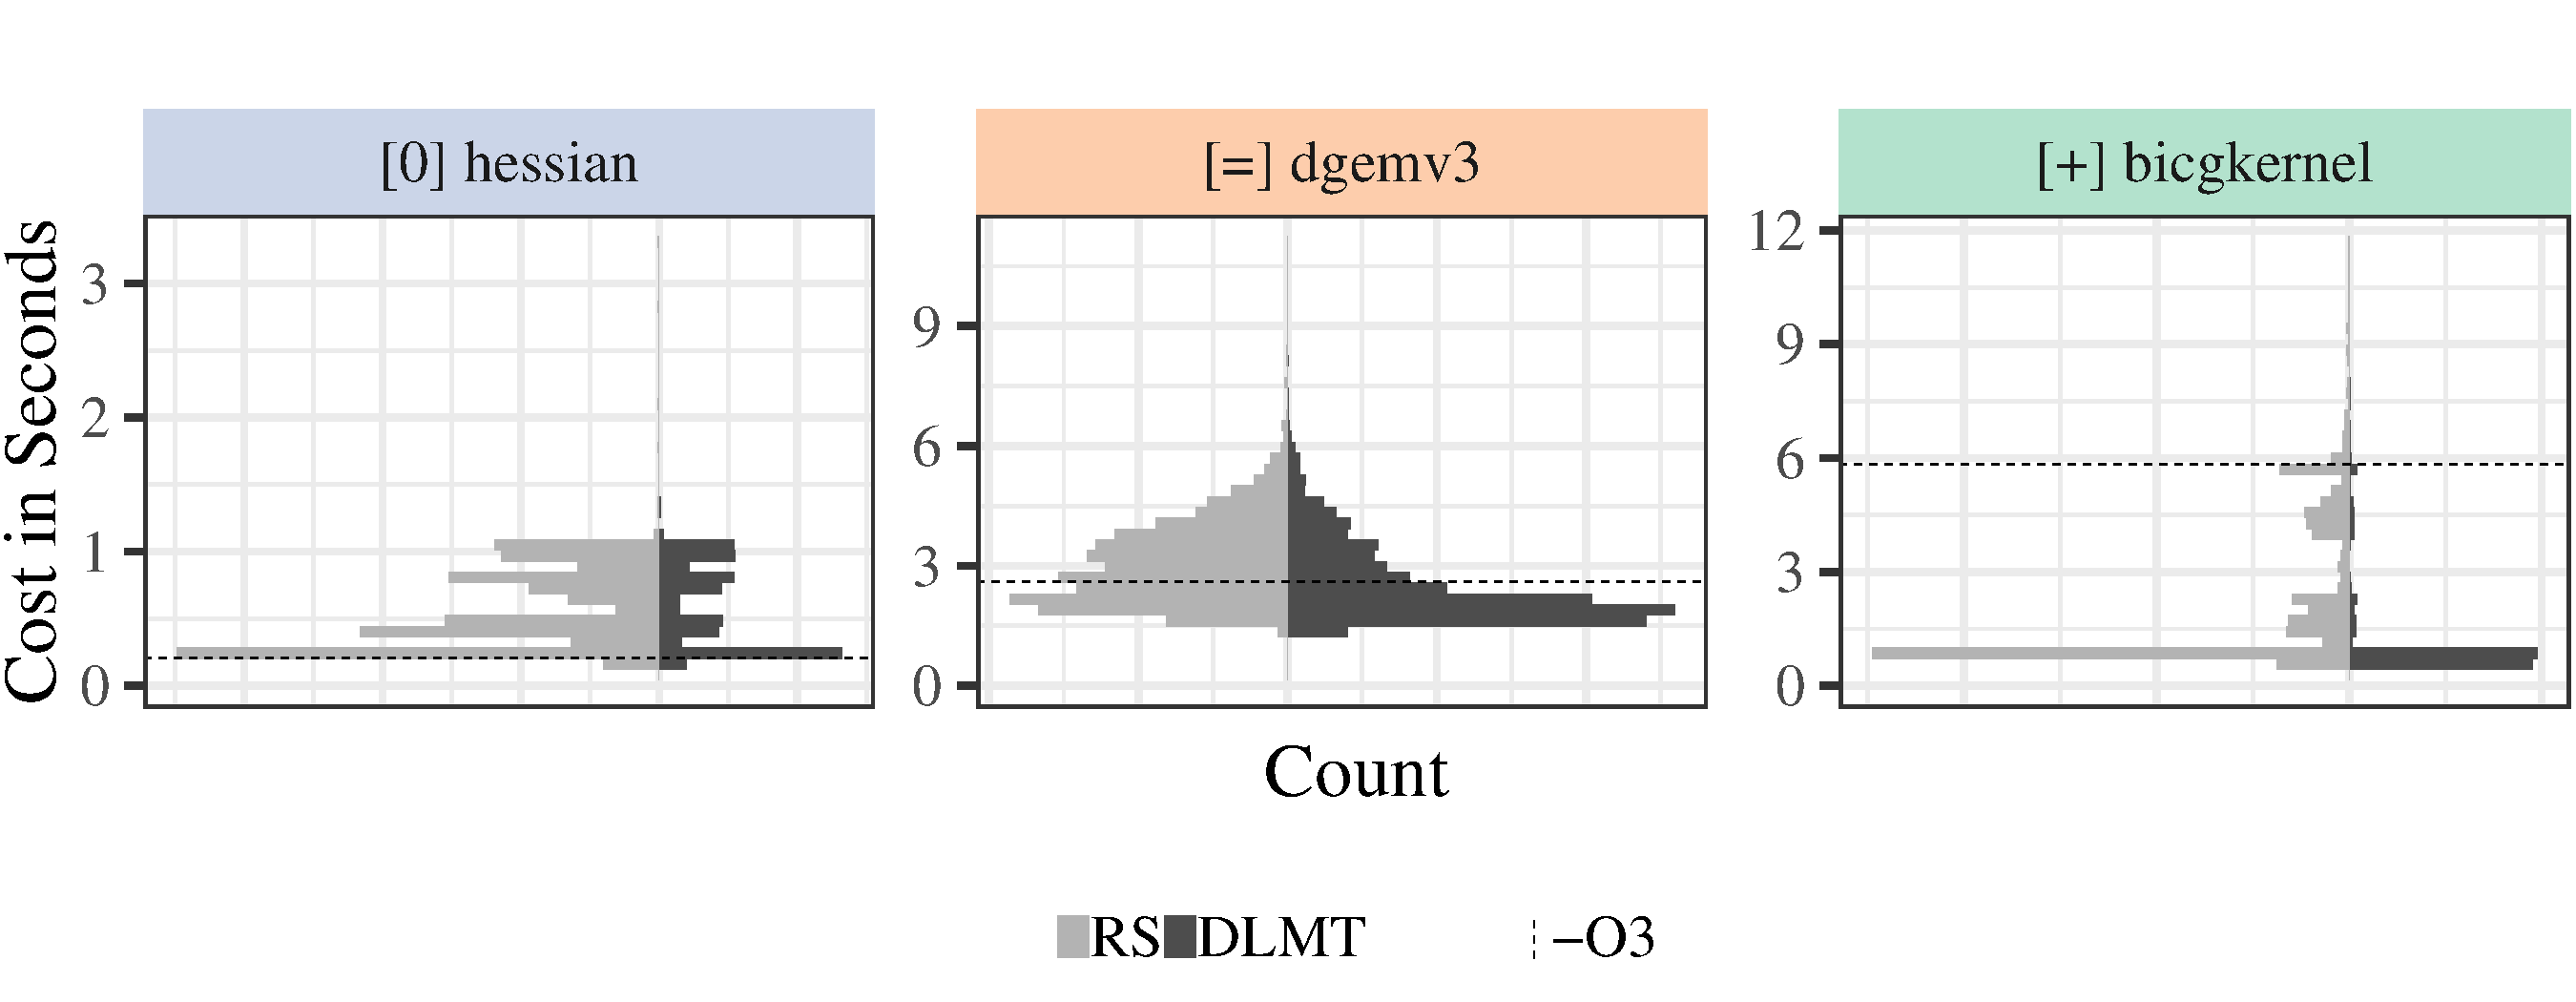
\includegraphics[width=.89\linewidth]{../../../img/split_histograms.pdf}
\end{center}
\end{center}
\end{frame}
\begin{frame}[label={sec:org78ff137}]{SPAPT: Summary}
\begin{columns}
\begin{column}{0.5\columnwidth}
\begin{block}{Experimental Settings}
\begin{itemize}
\item Using the \alert{same model for all applications}
\item Fixed \alert{number of iterations}
\item \alert{Automated approach}
\end{itemize}
\end{block}
\end{column}

\begin{column}{0.5\columnwidth}
\begin{block}{Summary}
\begin{itemize}
\item Performance \alert{similar to random sampling}
\item Using \alert{less points}
\end{itemize}
\end{block}
\end{column}
\end{columns}
\end{frame}

\begin{frame}[label={sec:orgbc3bbe6}]{Conclusion}
\begin{columns}
\begin{column}{0.5\columnwidth}
\begin{block}{Summary}
\vspace{.2cm}

Our approach uses:

\begin{itemize}
\item \alert{Efficient experimental designs} to overcome issues related to \alert{exponential growth}, \alert{geometry}, and \alert{measurement time}
\item \alert{Analysis of variance} to find \alert{relevant parameters}
\item \alert{User input} to guide optimization
\end{itemize}

\vspace{2cm}
\end{block}
\end{column}
\begin{column}{0.5\columnwidth}
\begin{block}{Perspectives}
\begin{itemize}
\item Explore \alert{tailored models} for each application
\item Leverage \alert{user input} and \alert{analysis}
\item Use our approach to \alert{autotune industrial-level FPGA applications}
\end{itemize}
\end{block}
\end{column}
\end{columns}
\end{frame}

\maketitle
\end{document}